\documentclass[a4paper,14pt]{extarticle}

\usepackage[left=30mm, right=10mm, top=20mm, bottom=20mm]{geometry}

\usepackage[T2A]{fontenc}
\usepackage[utf8]{inputenc}
\usepackage[russian]{babel}
\usepackage{tempora}
\usepackage{type1cm}
\usepackage{indentfirst}

\usepackage{minted}
\usepackage{xcolor}

\usepackage{siunitx}
\usepackage{booktabs}
\usepackage{multirow}

\usepackage{csquotes}
\usepackage[
    parentracker=true,
    backend=biber,
    style=gost-numeric,
    sorting=nty
]{biblatex}

\usepackage[nodisplayskipstretch]{setspace}
\usepackage[none]{hyphenat}
\usepackage{fancyhdr}
\usepackage{titlesec}
\usepackage{tocloft}

\usepackage{amssymb}
\usepackage{amsmath}
\usepackage{tikz}
\usepackage{pgfplots}
\usepackage{graphicx}
\usepackage{caption}
\usepackage{subcaption}
\usepackage[hidelinks]{hyperref}
\usepackage[russian]{cleveref}
\usepackage{bookmark}

\pgfplotsset{compat=1.18}

\onehalfspacing
\sloppy

\pagestyle{fancy}
\fancyhf{}
\fancyfoot[R]{\thepage}
\renewcommand{\headrulewidth}{0pt}

\definecolor{codebg}{rgb}{0.12,0.12,0.14}
\definecolor{codeframe}{rgb}{0.40,0.40,0.45}
\definecolor{keywordcolor}{rgb}{0.45,0.65,1.0}
\definecolor{stringcolor}{rgb}{1.0,0.55,0.45}
\definecolor{commentcolor}{rgb}{0.55,0.75,0.60}
\definecolor{textcolor}{rgb}{0.90,0.90,0.90}

\renewcommand{\theFancyVerbLine}{
	\sffamily\small\color{black}\arabic{FancyVerbLine}
}

\setminted{
    bgcolor=codebg,
	fillcolor=codebg,
	framesep=1em,
	frame=single,
    rulecolor=\color{codeframe},
    fontsize=\normalsize,
    baselinestretch=1.1,
    linenos,
    numbersep=6pt,
    tabsize=4,
    breaklines,
    breakbytoken,
	breaksymbolleft={},
    autogobble,
    showspaces=false,
    showtabs=false,
}

\usemintedstyle{lightbulb}
\setmintedinline{
    bgcolor=codebg
}

\makeatletter
\setlength{\@fptop}{0pt}
\setlength{\@fpsep}{8pt}
\setlength{\@fpbot}{0pt plus 1fil}
\makeatother

\newcommand{\circledequals}{\mathbin{\tikz \node[draw,circle,inner sep=1pt] {$=$};}}

\begin{document}
    \tableofcontents
    \thispagestyle{empty}

    \newpage
    \section{Постановка задачи}
    \subsection{Бизнес-контекст и цель проекта}
    В рамках подготовки и адаптации фильмов к требованиям целевых возрастных категорий и регламентам дистрибуции возникает необходимость регулярной модерации поступающих видеоматериалов.
    \textbf{Цель проекта} -- разработать пайплаин обработки видеоконтента, который на основе имеющегося датасета с экспертной разметкой обучается самостоятельно выявлять и модифицировать нежелательный контент в новых поступлениях фильмов.

    Внедряемая система должна обеспечивать автоматизированное выполнение двух ключевых операций над каждым новым фильмом:
    \begin{itemize}
        \item обнаружение и удаление сцен, содержание которых не соответствует заданному возрастному рейтингу;
        \item обнаружение в кадре изображений оружия и их блюра.
    \end{itemize}

    \subsection{Формализация исходных данных и целевого результата}
    Имеющийся в распоряжении компании размеченный датасет $D$ представляет собой набор полнометражных фильмов, для каждого из которых заданы:
    \begin{itemize}
        \item исходный медиафайл $X_i$, представляющий видеоряд;
        \item временная разметка запрещённых сцен $Y_{i,\text{scene}}$, определяющая границы интервалов, подлежащих удалению;
        \item пространственно-временная разметка оружия $Y_{i,\text{weapon}}$, фиксирующая номер кадра и координаты ограничивающей рамки для каждого экземпляра оружия.
    \end{itemize}

    В продуктовом режиме на вход системы поступает новый неразмеченный фильм $X_{\text{new}}$. 
    Результатом работы пайплаина является $Y_{\text{new}} = \{ Y_{\text{scene}_{\text{new}}}, Y_{\text{weapon}_{\text{new}}} \}$, в котором удалены размечены эпизоды и области с оружием.

    \subsection{Математическая формализация задачи}
    $D$ -- текущий датасет: $D = \{ (X_i, Y_i) ~~ | ~~ i = \overline{1, N} \}$, $X_i$ -- видеоряд, $Y_i$ -- набор разметок, $N$ -- количество видеорядов в датасете. \\
    $
    Y_i = \{ (Y_{i,\text{scene}}, Y_{i,\text{weapon}}) \} \\
    Y_{i,\text{scene}} = \{(t_{ij}^{\text{start}}, t_{ij}^{\text{end}}) ~~|~~ t_{ij}^{\text{start}}, t_{ij}^{\text{end}} \in \mathbb{R}, ~ t_{ij}^{\text{start}} < t_{ij}^{\text{end}}, ~ j = \overline{1, s_i}, ~ s_i \in \mathbb{N} \},
    $
    где $s_i$ -- количество запрещённых сцен в видеоряде $X_i$ \\
    $
    Y_{i,\text{weapon}} = \{ (c_{ij}, b_{ij}) ~~|~~ c_{ij} \in \mathbb{N}, ~ j = \overline{1, \omega_i}, ~ \omega_i \in \mathbb{N} \},
    $
    где $\omega_i$ -- количество кадров с оружием в видеоряде $X_i$ \\
    $
    b_{ij} = \{ (x_{ij}, y_{ij}), (w_{ij}, h_{ij}) ~~|~~ x_{ij}, y_{ij} \geq 0, ~ w_{ij}, h_{ij} > 0 \},
    $
    где $x_{ij}, y_{ij}$ -- координаты верхнего левого угла рамки, $w_{ij}, h_{ij}$ -- ширина и высота рамки.

    Пусть у нас имеются модели $M_{\text{scene}}(\cdot\,; \theta_{\text{scene}})$ и $M_{\text{weapon}}(\cdot\,; \theta_{\text{weapon}})$ с векторами обучаемых параметров $\theta_{\text{scene}}$ и $\theta_{\text{weapon}}$ для обнаружения запрещённых сцен и объектов оружия соответственно. На вход каждой модели подаётся видеоряд $X_i$ целиком:
    \begin{align*}
        \hat{Y}_{i,\text{scene}} &= M_{\text{scene}}(X_i; \theta_{\text{scene}}) = \big\{ (\hat{t}_{im}^{\text{start}}, \hat{t}_{im}^{\text{end}}, \hat{p}_{im}^{\text{scene}}) \big\}_{m=1}^{\hat{s}_i}, \\
        \hat{Y}_{i,\text{weapon}} &= M_{\text{weapon}}(X_i; \theta_{\text{weapon}}) = \big\{ (\hat{t}_{im}, \hat{b}_{im}, \hat{p}_{im}^{\text{weapon}}) \big\}_{m=1}^{\hat{\omega}_i},
    \end{align*}
    где $\hat{p}_{im}^{\text{scene}}, \hat{p}_{im}^{\text{weapon}} \in [0, 1]$ -- оценки уверенности моделей в соответствующих предсказаниях, $\hat{s}_i$ и $\hat{\omega}_i$ -- количество предсказанных интервалов сцен и рамок оружия для видеоряда $X_i$.

    Разделяем датасет $D$ на 3 непересекающиеся подмножества:
    \begin{itemize}
        \item $D_{\text{train}}$ -- обучающий датасет;
        \item $D_{\text{val}}$ -- валидационный датасет;
        \item $D_{\text{test}}$ -- тестовый датасет.
    \end{itemize}

    Для сравнения предсказанного набора интервалов $\hat{Y}_{i,\text{scene}}$ с истинной разметкой $Y_{i,\text{scene}}$ определяется функция потерь $\mathcal{L}_{\text{scene}}(\hat{Y}_{i,\text{scene}}, Y_{i,\text{scene}})$, объединяющая ошибку классификации наличия запрещённого контента и ошибку определения временных границ.

    Функция потерь $\mathcal{L}_{\text{weapon}}(\hat{Y}_{i,\text{weapon}}, Y_{i,\text{weapon}})$ оценивает точность обнаружения оружия по всему видеоряду $X_i$.

    Обучение моделей формулируется как задача минимизации ошибки на обучающей выборке $D_{\text{train}}$ по параметрам $\theta_{\text{scene}}$ и $\theta_{\text{weapon}}$:
    \begin{align*}
        \theta_{\text{scene}}^* &= \arg\min_{\theta_{\text{scene}}} \frac{1}{|D_{\text{train}}|} \sum_{(X_i, Y_i) \in D_{\text{train}}} \mathcal{L}_{\text{scene}}\big(M_{\text{scene}}(X_i; \theta_{\text{scene}}), Y_{i,\text{scene}}\big), \\
        \theta_{\text{weapon}}^* &= \arg\min_{\theta_{\text{weapon}}} \frac{1}{|D_{\text{train}}|} \sum_{(X_i, Y_i) \in D_{\text{train}}} \mathcal{L}_{\text{weapon}}\big(M_{\text{weapon}}(X_i; \theta_{\text{weapon}}), Y_{i,\text{weapon}}\big).
    \end{align*}
    Подбор гиперпараметров и критерий остановки обучения определяются по целевым метрикам качества на валидационной выборке $D_{\text{val}}$, а финальная оценка эффективности моделей выполняется на тестовой выборке $D_{\text{test}}$.

    \section{Технические метрики и функции потерь}
    Качество моделей оценивается на тестовой выборке фильмов с экспертной разметкой. 
    Для обеих задач используются точность (Precision) и полнота (Recall). 
    Эти метрики позволяют учитывать как пропуск нежелательного контента, так и ошибочную обработку допустимого материала.

    Для удаления запрещённой сцены система определяет временной интервал $[t_i^{\text{start}}, t_i^{\text{end}}]$, где $t_i^{\text{start}}$ и $t_i^{\text{end}}$ -- таймкоды начала и конца сцены. 
    После утверждения интервала соответствующий фрагмент синхронно вырезается из всех медиадорожек.

    Для размытия оружия детектор определяет в кадре ограничивающую рамку (bounding box) с координатами $B=(x_{\min}, y_{\min}, x_{\max}, y_{\max})$. 
    Пара $(x_{\min}, y_{\min})$ задаёт левый верхний угол рамки, а $(x_{\max}, y_{\max})$ -- правый нижний. 
    Координаты измеряются в пикселях от левого верхнего угла кадра. 
    Модуль размытия обрабатывает прямоугольную область между этими точками.

    \subsection{Обнаружение и удаление запрещённых сцен}
    Предсказанные интервалы удаления сравниваются с экспертными интервалами $Y_{\text{scene}}$. 
    Величина $TP$ обозначает длительность их пересечения, $FP$ --- длительность ошибочно отмеченного допустимого материала, а $FN$ --- длительность пропущенного запрещённого материала. 
    Эти значения суммируются по фильмам тестовой выборки:
    \[
        \mathrm{Precision} = \frac{TP}{TP+FP},
        \qquad
        \mathrm{Recall} = \frac{TP}{TP+FN}.
    \]
    Precision показывает, какая доля отмеченного для удаления материала действительно подлежит удалению. 
    Recall показывает, какая доля общей длительности запрещённых сцен обнаружена.

    Границы сцены проверяются по таймкодам исходного фильма. 
    Например, если конец сцены определён верно, а начало отмечено на два кадра раньше, длительность этих кадров учитывается в $FP$. 
    Если начало отмечено на два кадра позже, их длительность учитывается в $FN$.

    \subsection{Обнаружение оружия и определение области размытия}
    После трекинга рамка $B$, переданная на размытие, сравнивается с экспертной рамкой $m_i$ в том же кадре. 
    Степень совпадения оценивается по метрике Intersection over Union (IoU):
    \[
        \mathrm{IoU}(B,m_i) = \frac{|B \cap m_i|}{|B \cup m_i|}.
    \]
    IoU учитывает как неполное покрытие экспертной рамки, так и выход за её границы. 
    Принят порог $\mathrm{IoU} \geq 0{,}5$: площадь пересечения должна составлять не менее половины площади объединения рамок.

    Каждая рамка может входить только в одну совпавшую пару. 
    Для расчёта Precision и Recall величина $TP$ обозначает число совпавших пар, $FP$ --- число лишних предсказанных рамок, а $FN$ --- число пропущенных экспертных рамок.

    Смещение отдельной границы определяется по разности координат. 
    Например, если у экспертной рамки $x_{\max}=200$, а у предсказанной $x_{\max}=202$, правая граница области размытия смещена на два пикселя вправо. 
    Такое смещение возможно даже при высоком IoU.

    \subsection{Функции потерь}

    Для обучения модели обнаружения сцен используется взвешенная бинарная кросс-энтропия. 
    Каждому анализируемому моменту присваивается метка 1 внутри экспертного интервала удаления и 0 за его пределами. 
    Повышенный вес положительного класса учитывает малую долю запрещённых сцен в общем хронометраже.

    Для детектора оружия выбрана составная функция потерь
    \[
        L_{\text{weapon}} = L_{\text{BCE}} + \lambda L_{\text{Smooth L1}}.
    \]
    Бинарная кросс-энтропия $L_{\text{BCE}}$ оценивает ошибку классификации области как оружия или фона. 
    Для областей, сопоставленных с экспертными рамками оружия, $L_{\text{Smooth L1}}$ учитывает отклонения предсказанных координат от экспертных. 
    Коэффициент $\lambda$ задаёт вес ошибки координат при обучении.


    \section{System design}
    \begin{figure}[h]
        \centering
        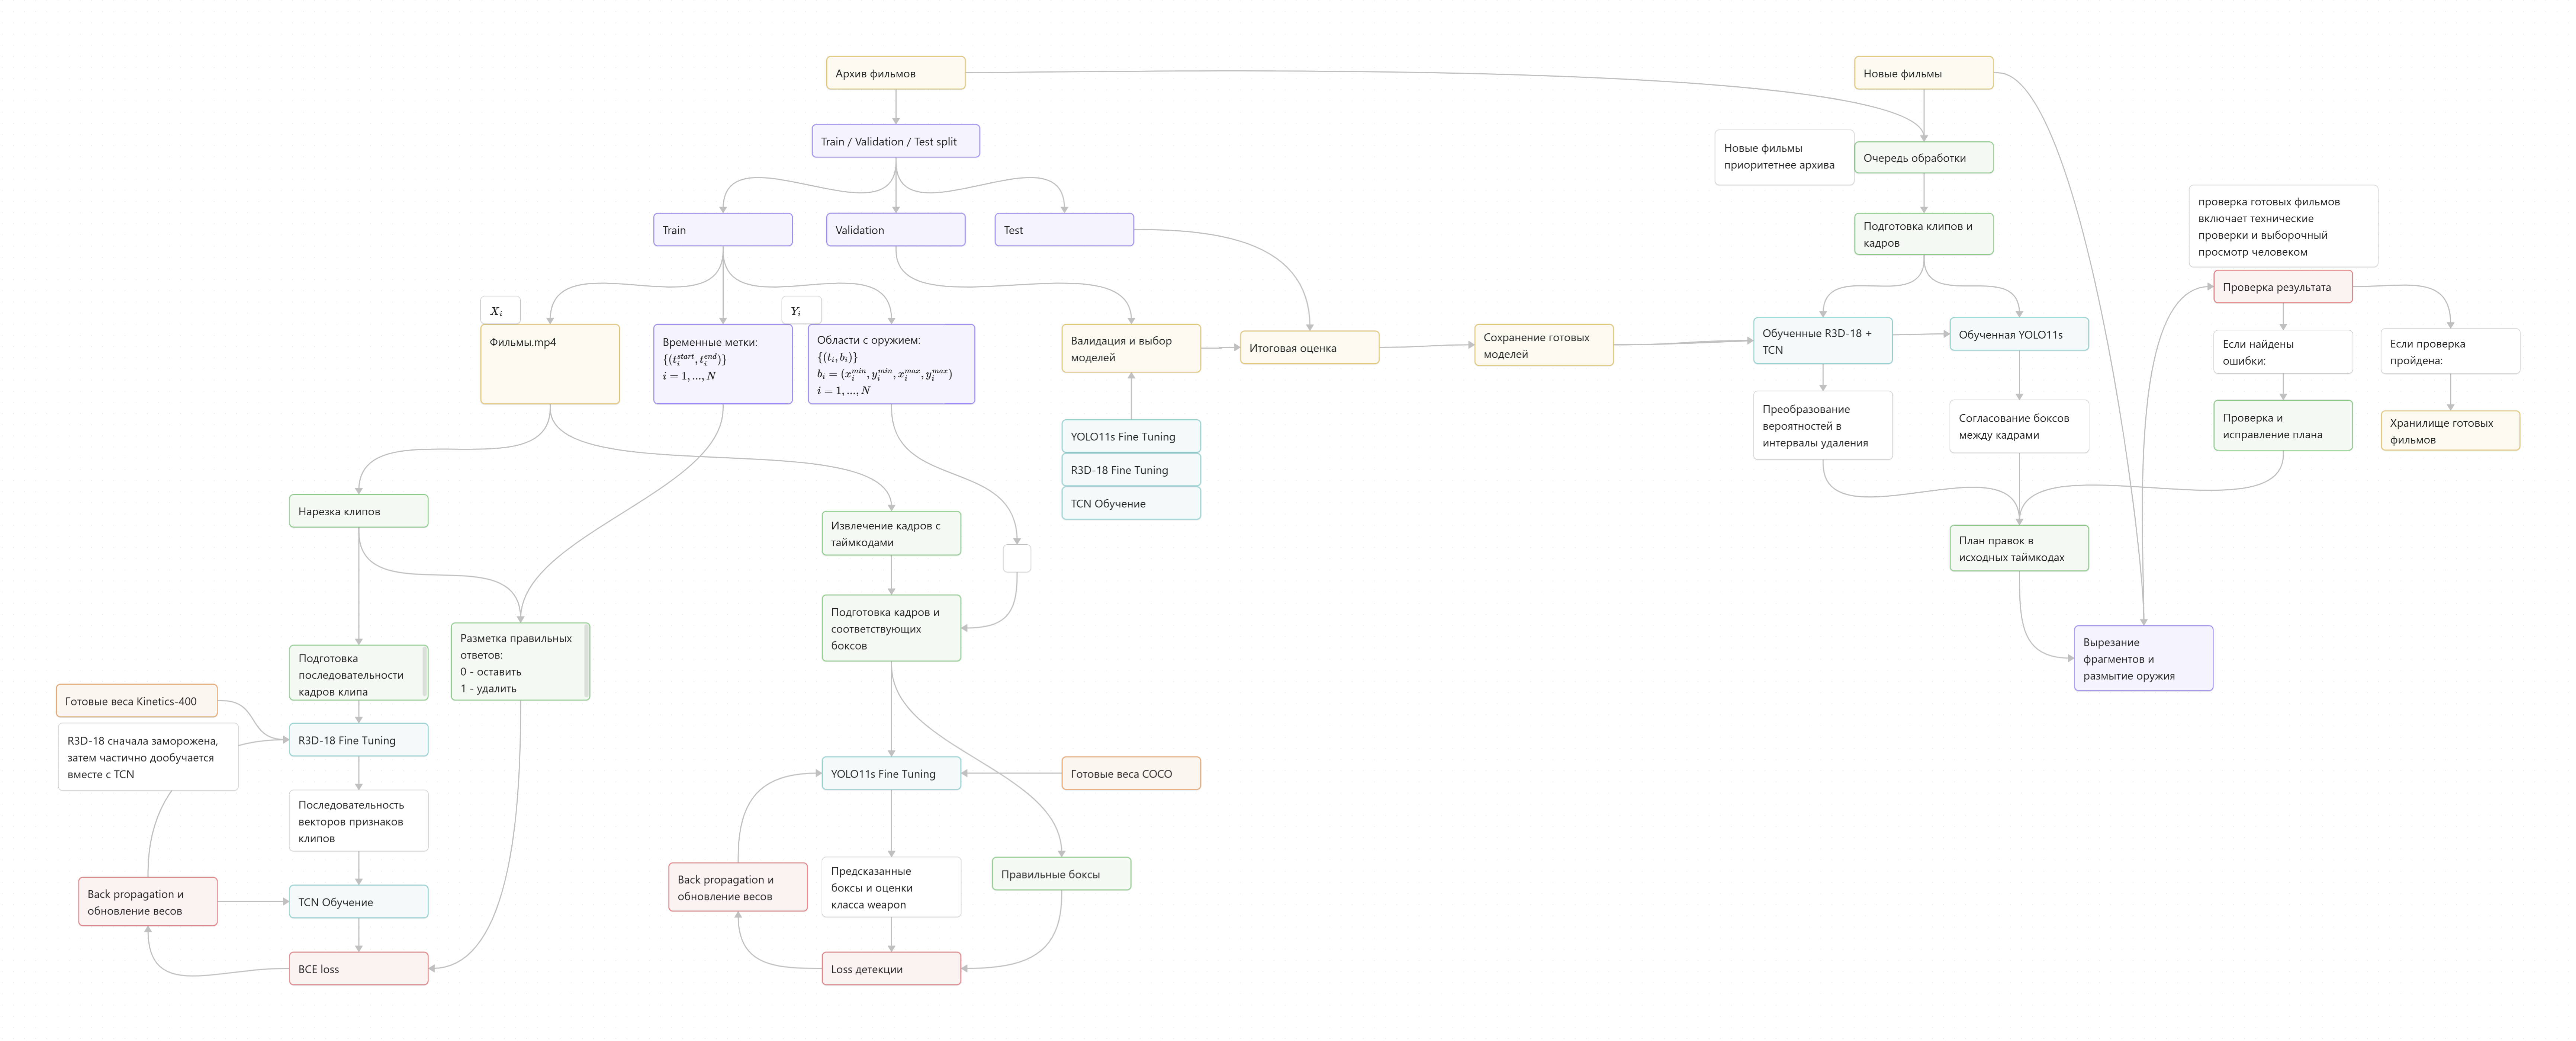
\includegraphics[width=\textwidth]{system.png}
    \end{figure}

    Система выполняет предварительную обработку фильмов по заданной политике: удаляет сексуальные сцены, включая прелюдию, и размывает изображения оружия. 
    Обычные поцелуи сохраняются. Архитектура включает обучение моделей, их независимую проверку и обработку видеоматериалов. 
    Используются две отдельные модели: для определения временных интервалов удаления и для обнаружения оружия.

    Источником обучающих данных является архив фильмов с размеченными интервалами удаления и ограничивающими прямоугольниками оружия. 
    Архив разделяется на train, validation и test по фильмам до извлечения кадров и клипов. 
    Видео и соответствующая разметка всегда принадлежат одной части; дубликаты и версии одного фильма также группируются вместе. 
    Это предотвращает попадание практически одинаковых примеров в обучение и проверку.

    Для поиска интервалов удаления используется связка R3D-18 и TCN. 
    Фильм разбивается на короткие перекрывающиеся клипы с сохранением исходных таймкодов. 
    R3D-18 с весами Kinetics-400 извлекает признаки каждого клипа, а TCN анализирует их последовательность и выдаёт вероятности удаления для соответствующих временных позиций. 
    Целевые метки формируются по попаданию центра клипа в размеченный интервал; сам клип предоставляет окружающий контекст. 
    Обучение использует бинарную кросс-энтропию. 
    Сначала R3D-18 заморожена и обучается новая TCN, затем последние блоки R3D-18 дообучаются совместно с TCN.

    Оружие обнаруживается детектором YOLO11s, предобученным на COCO и дообученным на архивных кадрах для класса weapon. 
    Подготовка данных включает сопоставление кадров с разметкой и согласованное преобразование изображений и координат прямоугольников. 
    Используются как кадры с оружием, так и кадры без него. 
    Функция ошибки учитывает классификацию и локализацию объектов. 
    Поскольку разметка содержит прямоугольники, размытие применяется к прямоугольной области; пиксельная сегментация в выбранной архитектуре не используется.

    На validation выбираются версии весов, пороги и параметры постобработки. 
    После фиксации конфигурации проводится итоговая оценка на test без обновления весов и подбора настроек. 
    Вместе с моделями сохраняются параметры подготовки входов, постобработки и сведения о версии данных.

    Архивные и новые фильмы поступают в общую очередь обработки. 
    Новые поступления имеют повышенный приоритет, при этом часть ресурсов выделяется архиву для обеспечения его полной обработки. 
    Применяются те же правила подготовки входов, что и при проверке моделей. 
    Вероятности временной модели преобразуются в интервалы удаления. 
    Детекции оружия согласовываются между соседними кадрами для уменьшения мигания размытия; при смене плана связь объектов сбрасывается. 
    Результаты объединяются в план правок с исходными таймкодами и координатами.

    Компонент монтажа применяет план к оригиналу: размывает оружие в сохраняемых кадрах, удаляет выбранные интервалы из видео и всех аудиодорожек, пересчитывает субтитры. 
    Оригиналы сохраняются, результат записывается отдельной версией. 
    Готовые файлы проходят технические проверки, а качество обработки дополнительно оценивается выборочным просмотром человеком. 
    При обнаружении ошибок план исправляется и монтаж повторяется. 
    Очередь хранит состояния заданий и поддерживает повторные попытки при технических сбоях.

    \section{Бизнес метрики}
    Бизнес-метрики предназначены для оценки эффективности разработанной модели обработки видеоконтента с точки зрения полноты обработки фильмов, соблюдения сроков, временных и финансовых затрат, а также стабильности работы системы. 
    В отличие от технических метрик, которые оценивают качество работы отдельных моделей обнаружения сцен и оружия, бизнес-метрики позволяют оценить результативность всего процесса обработки видеоматериалов.

    Выбранные показатели учитывают два направления эксплуатации системы:
    \begin{itemize}
        \item Первоначальная обработка существующего архива фильмов;
        \item Регулярная обработка новых поступлений.
    \end{itemize}

    \subsection{Age Rating Compliance Rate - соответствие внутренним требованиям возрастной категории}
    Показатель отражает долю обработанных фильмов, которые соответствуют внутренним требованиям проекта для версии контента 16+. 
    Соответствие определяется по результатам итоговой проверки адаптированного фильма: нежелательные сцены должны быть удалены, а изображения оружия - размыты в соответствии с заданными правилами.
    \begin{equation*}
        \displaystyle ARCR = \frac{N_{\text{compliant}}}{N_{\text{processed}}} \cdot 100 \%,
    \end{equation*}
    где $N_{\text{compliant}}$ -- количество обработанных фильмов, прошедших итоговую проверку и соответствующих установленным требованиям, $N_{\text{processed}}$ -- общее количество фильмов, прошедших полный цикл обработки.

    Она позволяет оценить конечный результат работы всего модели, а не только качество отдельных моделей. 
    Важно, чтобы итоговый видеофайл действительно соответствовал установленным требованиям проекта.

    \subsection{Content Processing Coverage - полнота обработки каталога}
    Показатель характеризует долю фильмов из общего каталога, для которых успешно сформирована адаптированная версия. 
    Фильм считается обработанным только после завершения всех этапов модели и формирования итогового медиафайла.
    \begin{equation*}
        \displaystyle C_{\text{processing}} = \frac{N_{\text{processed}}}{N_{\text{total}}} \cdot 100 \%,
    \end{equation*}
    где $N_{\text{processed}}$ -- количество фильмов, успешно прошедших полный цикл обработки, $N_{\text{total}}$ -- общее количество фильмов, подлежащих обработке.

    Она позволяет оценить, какая часть существующего архива уже адаптирована, а также контролировать полноту обработки новых поступлений.
    Это особенно важно, поскольку система должна работать не только с отдельными фильмами, но и с большим объёмом накопленного видеоконтента.

    \subsection{Processing Time per Movie - время обработки одного фильма}
    Метрика определяет продолжительность полного цикла обработки одного фильма - от фактического начала работы модели до формирования готовой адаптированной версии.
    \begin{equation*}
        \displaystyle T_{\text{processing}} = t_{\text{ready}} - t_{\text{start}},
    \end{equation*}
    где $t_{\text{ready}}$ -- время фактического начала обработки фильма, $t_{\text{start}}$ -- время формирования готового выходного файла.

    Для оценки общей производительности системы рекомендуется использовать медианное время обработки по всему набору фильмов. 
    Дополнительно можно учитывать 95-й перцентиль (P95), позволяющий выявлять фильмы, обработка которых занимает значительно больше времени.

    Продолжительность обработки напрямую влияет на возможность системы справляться с большими объёмами видеоматериалов. 
    Показатель позволяет оценить затраты времени на адаптацию одного фильма и определить, насколько быстро система может обрабатывать новые поступления.

    \subsection{SLA Compliance Rate - соблюдение сроков обработки}
    Метрика показывает долю фильмов, успешно обработанных в пределах заранее установленного срока.
    \begin{equation*}
        \displaystyle SLA = \frac{N_{\text{on-time}}}{N_{\text{due}}} \cdot 100 \%,
    \end{equation*}
    где $N_{\text{on-time}}$ -- количество фильмов, обработанных до установленного срока, $N_{\text{due}}$ -- количество фильмов, срок обработки которых наступил в рассматриваемом периоде.

    Для новых поступлений срок определяется требованиями к подготовке фильма перед публикацией адаптированной версии.
    Для существующего архива - утверждённым графиком пакетной обработки.

    Она позволяет оценить, насколько надёжно система выполняет задачи в установленные сроки. 
    В отличие от времени обработки одного фильма, данный показатель оценивает способность всего процесса укладываться в заданные временные ограничения.

    \subsection{Cost per Movie - стоимость обработки одного фильма}
    Показатель определяет средние затраты, необходимые для полной обработки одного фильма. 
    Учитываются ресурсы, используемые на всех этапах работы модели.
    \begin{equation*}
        \displaystyle Cost_{\text{movie}} = \frac{C_{\text{total}}}{N_{\text{completed}}},
    \end{equation*}
    где $C_{\text{total}}$ -- общие затраты на обработку фильмов за выбранный период, $N_{\text{completed}}$ -- количество успешно обработанных фильмов за тот же период.

    В общие затраты могут входить расходы на вычислительные ресурсы, хранение и передачу данных, а также повторные запуски обработки и ручную проверку результатов, если она предусмотрена процессом.

    Обработка полнометражных фильмов требует значительных вычислительных ресурсов и времени.
    Данный показатель позволяет оценить затраты на адаптацию одного фильма и определить ресурсную эффективность разработанного решения.

    \subsection{Reprocessing Rate - доля фильмов, требующих повторной обработки}

    Показатель отражает долю фильмов, для которых потребовался повторный запуск модели из-за сбоев обработки, ошибок формирования выходного файла или проблем при сохранении результата.
    \begin{equation*}
        \displaystyle R_{\text{reprocessing}} = \frac{N_{\text{reprocessing}}}{N_{\text{started}}} \cdot 100 \%,
    \end{equation*}
    где $N_{\text{reprocessing}}$ -- количество фильмов, для которых потребовался хотя бы один повторный запуск обработки, $N_{\text{started}}$ -- общее количество фильмов, обработка которых была начата за рассматриваемый период.

    При расчёте каждый фильм учитывается только один раз независимо от количества повторных запусков.

    Повторная обработка приводит к дополнительным затратам вычислительных ресурсов и увеличению времени подготовки фильмов. 
    Показатель позволяет оценить стабильность работы модели и определить, насколько часто процесс требует повторного выполнения из-за технических проблем.

    \subsection{Порядок оценки эффективности}
    Для оценки эффективности разработанного модели бизнес-метрики рассматриваются в совокупности, поскольку каждая из них характеризует отдельную сторону процесса обработки видеоконтента.

    При обработке существующего архива основное внимание уделяется полноте обработки каталога (Content Processing Coverage), времени обработки одного фильма (Processing Time per Movie) и стоимости обработки (Cost per Movie). 
    Эти показатели позволяют оценить скорость адаптации накопленного контента и необходимые для этого ресурсы. 
    При работе с новыми поступлениями дополнительно учитываются соблюдение установленных сроков (SLA Compliance Rate), соответствие итоговых фильмов внутренним требованиям проекта (Age Rating Compliance Rate) и доля повторных запусков обработки (Reprocessing Rate).

    Для оценки эффективности автоматизации также используется показатель сокращения времени обработки относительно ручного процесса (Processing Time Reduction). 
    Он позволяет сравнить время выполнения одинаковых операций вручную и с помощью разработанной модели, оценив полученное сокращение времени.

    Для расчёта метрик система должна фиксировать время поступления и начала обработки, время завершения, статус выполнения, количество повторных запусков, вычислительные затраты и результаты итоговой проверки. 
    Это позволит отслеживать эффективность работы модели на протяжении всего периода эксплуатации.

    Для Age Rating Compliance Rate, Content Processing Coverage и SLA Compliance Rate предпочтительны более высокие значения, тогда как Processing Time per Movie, Cost per Movie и Reprocessing Rate должны стремиться к снижению. 
    При этом сокращение времени и стоимости обработки не должно приводить к ухудшению качества итоговых видеофайлов. 
    Для Processing Time Reduction, напротив, желательны более высокие значения, поскольку они свидетельствуют о сокращении времени обработки по сравнению с ручным процессом.

    Целевые значения показателей устанавливаются после пробного запуска системы на тестовой группе фильмов с учётом фактической производительности и потребления вычислительных ресурсов.

    \section{Распределение задач}
    Кулахсзян Сергей составил постановку задач и математическую формулировку задания.

    Ершова Валерия описала технические метрики и функции потерь.

    Захватов Дмитрий составил system design.

    Бобрунов Егор описал бизнес метрики.
\end{document}